\RequirePackage[hyphens]{url}

\documentclass[sigconf]{acmart}

\usepackage{graphicx}
\usepackage{hyperref}
\usepackage{todonotes}

\usepackage{endfloat}
\renewcommand{\efloatseparator}{\mbox{}} % no new page between figures

\usepackage{booktabs} % For formal tables

\settopmatter{printacmref=false} % Removes citation information below abstract
\renewcommand\footnotetextcopyrightpermission[1]{} % removes footnote with conference information in first column
\pagestyle{plain} % removes running headers

\newcommand{\TODO}[1]{\todo[inline]{#1}}
\newcommand{\DONE}[1]{DONE: \todo[inline,color=green!30]{#1}}

\begin{document}
\title{The Intersection of Big Data and IoT}

\author{Peter Russell}
\affiliation{%
  \institution{Indiana University}
}
\email{petrusse@iu.edu}

\begin{abstract}

Big Data and IoT share a symbiotic relationship with one another that is leading to incredible innovations that were inconceivable just 18 years ago. As a result of this relationship, it has become easier than ever for individuals to customize and monitor various elements of their life if they choose to do so. We examine a few of the emerging technologies within IoT, highlight some of the most interesting current use cases and show how Big Data plays a role before presenting a challenges that lie ahead for the technology. Finally, a demonstrative project is undertaken via the Raspberry Pi to illustrate how accessible IoT has become to leverage Big Data analysis.
\end{abstract}

\keywords{i523, HID 334, Edge Computing, Raspberry Pi, IoT}

\maketitle

\section{Introduction}
In 2020, it is estimated that 95 percent of electronics will contain IoT technology \cite{gartner95}. This technology, commonly abbreviated for the ``Internet of Things'', is expected to be so pervasive due to how the technology is defined and how impactful it has already become. 

At the highest level, IoT is intended to describe devices that collect and relay information via the Internet. This leaves IoT is broadly defined in the type of application, which could come in the form of a phone, vehicle, a home device like a thermostat or television, but the technology is rather specific in its intended application. That is, these devices are generally made to serve a single purpose and they are extremely adept at that function. In its most powerful applications, massive data sets are created from these individual IoT devices as they are synthesized together to meet a larger need, as we will see.  

The specific purpose of an IoT device is what differentiates this emerging technology from traditional computers. With the exception of recent developments, which will be explored in depth, early IoT devices were not intended to do the heavy computing like a computer would do. However, with rapid advancements in computing power and speed, the line differentiating the two has begun to blur. It is this increase in computing power that has lead IoT and Big Data to have a cooperative relationship to create some of the most exciting technology that's available today. 

The ability to collect and process more data has increased the utility of these devices as they're able to become more personalized, spurring tremendous growth recently, on the order of $30 \%$ annually. In 2017, it is expected to be the year that the number of IoT devices exceeds the number of people on Earth \cite{gartnerconnected}. This personalization is not without consequence though, which will be discussed later, so the relationship between IoT and Big Data is still evolving. 

To begin, we examine how the IoT came to be and continuously evaluate how it is integrated with Big Data. Next, we discuss high level implementations of these technologies in modern use before discussing some of the challenges the industry is facing. Finally, a demonstrative project will be outlined to show how Big Data can be used in an IoT device. 

\section{Emergence of IoT}
Given the massive and recent popularity of IoT, it might be a surprise to some to learn that this concept has been around since 1999. The idea to have multiple, remote devices communicating with one another to gain insights to a single problems was originally conceived by Kevin Ashton as a solution to supply chain management \cite{ashton}. At that point, the idea was ahead of its time as the internet was still gaining widespread adoption. However, as computing power and sensor costs have declined, IoT has become a main an indispensable aspect of most people's lives. One such example could be the integration of global positioning systems (GPS) into cellphones, which was introduced in just 2004, but has become a staple for nearly every phone released \cite{gps}.  
\subsection{What Defines IoT?}
Given the ascension of so many new technologies, it could be helpful to understand what technically constitutes an IoT device. This will be useful later when discussing the sample project undertaken and how these both relate to Big Data analysis. 

As stated earlier, at a high level, IoT is meant to describe devices that use internal or external sensors to connect to the Internet. These sensors could come in the form of the well known types, such as Wi-Fi, Bluetooth or RFID, to the perhaps less widely known, such as NFC (Near Field Communication) or Zigbee \cite{lopez}.

For these IoT devices, the Internet allows them to be tremendously influential in the advancement of Big Data by virtual of the amount of data the devices are able to collect. Specifically, IoT allows its users to quantify the world around them in ways that were previously not possible. For corporations, this yields tremendous advantages when it comes to business planning or equipment monitoring. For example, the average wind farm can generate 150,000 data points \emph{per second} and an engine turbine could give 500 gigabytes of data \cite{wind}. Additionally, for individuals, IoT enables people to monitor their activity on a daily basis through wearable fitness devices and customize their homes to save on energy consumption. It has been estimated the average household generates approximately 2,000 gigabytes of data a year and this is expected to increase five fold by 2020 \cite{iotdata}. As we will explore, this rapid increase is due in large part to the computing power of the individual devices, which allow for a greater volume of data to be collected. For example, if a person enjoys a simple bike ride and purchases the Garmin Edge 500 watch, on a single ride they are producing data across 61 different variables for statistics such as heart rate, elevation gained, cadence and output produced continuously for the duration of their ride \cite{garmin}.


\section{Edge Computing}

Edge computing is currently one of the most transformative technologies within IoT because it is changing the way the cloud is being utilized for Big Data analysis. 

The technology gains its name from how the information being processed by the device.  Prior to this recent innovation, information was gathered, sent to the cloud, processed there, and then the output is pushed back to the device. Namely, it was a centralized process. However, with edge computing, devices are more intelligent in what information they choose to send, providing a much more efficient process. For example, rather than having a camera monitor an area constantly, even when there is no motion, modern IoT cameras have been equipped with motion detection so information is only sent when there is something to actually record. Since this decision and processing is made on the actual device, it is considered to be at the \emph{edge} of the network.

Traditionally, IoT devices that were intended to work in conjunction, such as surveillance cameras, were simple in their functionality and storage. Namely, a group of cameras would record individually and send their results back to a central server. However, with improvements in image quality, this becomes a Big Data problem very quickly as these cameras are running around the clock collecting footage. In the historical model of a centralized server, this setup eventually creates problems as bandwith and storage issues emerge. These limitations are the problems that edge computing seeks to circumvent and has become a major catalyst in the growth of IoT devices \cite{edge}.   

One of the primary reasons this technology is possible is due to the dramatic decrease in computing costs. The demonstrative project that is undertaken later on is an example of how much computing power is now available in the simplest devices. For the cost of $\$10$ one can get a single-board computer with 1 GHz and 512 MB RAM through the Raspberry Pi.

For these reasons, this type of processing is close to becoming the majority as it is expected that by 2019, $45\%$ of all data collected by IoT devices will be processed at the edge of the network \cite{msft}. As we will see by examining several commercial use cases, this technology is allowing early adopters to gain unique, real-time insights through Big Data analytics into the health and composition of their businesses.

\subsection{Use Case: Fraud Detection}
Fraudulent transactions represent just $1\%$ of all transactions. However, while the relative size of these transactions to the overall market are small, their absolute impact is enormously detrimental to merchants and financial services companies. In 2015, total fraudulent transactions created damages of $\$22$ billion \cite{fraud}.

The economic impact of these transactions has given these companies a tremendous incentive to innovate their way out of this problem. The marriage of IoT and Big Data has now provided them the opportunity to have near real-time analytics, which is  necessity to effectively manage the problem. This is because the approval process for a transaction needs to be as close to instantaneous as possible. If shortcuts are taken in the analysis to increase speed, fraudulent transactions could slip through and not get flagged. IoT has helped make this trade-off between accuracy and speed less of an issue with new innovations, such as Visa's Ready program. 

Visa Ready is an innovative program enables payments through IoT for both security and convenience. Instead of traditional means of payment authorization, such as simply swiping your credit card at a vendor, IoT enables Visa to take advantage of improvements in biometric technology \cite{visa}. Visa has introduced multi-dimension verification through biometrics by letting users endorse a payment through their fingerprint, iris scan, face scan and even their voice \cite{biometric}. This type of technology is gaining adoption and there are expected for be 500 million devices with biometric sensors by 2018 and 26 billion by 2020 \cite{biometricsensors}. 

Complementing biometric data, as IoT devices become more mainstream, companies such as FICO are using behavioral data in fortifying their analysis of whether a transaction is fraudulent or not. This type of analysis is not new in and of itself as it has been established as a way to identify e-commerce fraud, but the application through IoT is providing a new dimension of analysis. Traditionally, behavior data was tracked to see how a user interacts with a website to reduce the number of false positives that get flagged, which could occur if a user was on a business trip and abruptly logged into their account to buy something from an IP in another country \cite{fico}. With IoT, this adds a tremendous amount of data to an already Big Data problem. Now these companies will have data on how users interact with an IoT device, such as how they hold their device in the case of a phone or their tendencies when using the keyboard \cite{biometricuses}. From a business perspective, this all occurs in the background without the user's experience without the product being interrupted. 

As a testament to the future of this relationship between IoT and Big Data, Visa has partnered with IBM. This was done in an effort to gain maximum benefit from this new biometric technology by leveraging Visa's payment infrastructure with IBM's efforts in artificial intelligence and Big Data analysis with IBM Watson \cite{ibmvisa}.

\subsection{Use Case: Autonomous Vehicles}

In many ways, autonomous vehicles represent the pinnacle of edge computing to date in unifying IoT and Big Data. Among its many goals, this technology is trying to use Big Data to resolve one of the modern tragic realities of our modern world - automobile fatalities.  Automobile accidents cause 1.2 million deaths a year, $94\%$ of which are attributable to human error \cite{fatalities}. For this reason, in conjunction with expected energy savings from car designs with this technology, the technology is expected to experience adoption rates that rivals mobile phones with significantly more impact \cite{autonomousimpact}. Traditional car makers have taken notice of the potential future and as an example of this, General Motors recently hired an Uber engineer to lead its self-driving initiative as the company's first ever Chief Technology Officer \cite{gmcto}.

The relation of autonomous cars to IoT via edge computing is once again out of necessity for real-time functionality. A car that processes it should stop two seconds too late is as potentially useful as never making the calculation in the first place, so timing is of the utmost importance. Amazing progress has already been made in the speed and complexity of calculations these autonomous vehicles can handle. One of the highest profile graphic card manufacturers, Nvidia, recently announced their system for autonomous vehicles at the rate of 320 \emph{trillion} operations a second \cite{nvidia}. Since these vehicles are equipped with various types of sensors to process its environment, this type of computing power is a near necessity to tackle this Big Data problem in real-time. 

Kevin Ashton's original vision for the IoT was to have an accurate view of inventory as RFID scanners synced over the Internet. In just 18 short years, these autonomous vehicles are achieving the same end of communication with one another on an incredible scale. In what's known as ``vehicle to vehicle communication'' autonomous cars will be able to send one another information on important considerations, such as road hazards or conditions, allowing GPS to take the most optimal route to its destination. Similarly, speed limit signs can take weather conditions into account, dynamically adjust the speed limit of the road and relay this to the car's navigation system \cite{vehiclecomm}. 

The companies that are pursuing autonomous driving are largely having the cars learn through the experiences of its sensors. It would be impossible to code every possible scenario a car could face, so instead, data is collected from the various sensors and loaded to the cloud for later analysis. For example, Tesla is accumulating a million miles worth of data across its sensors every 10 hours, leaving it with 780 million through mid-2016 \cite{tesla}. These sensors on board, which will be briefly described to show their application, are expected to generate 4,000 gigabytes of data \emph{daily} \cite{sensorcardata} \cite{howsensorswork}. This is another instance of the familiar union between IoT and Big Data. 

\subsection{Use Case: Health Care}

The United States, like the world as a whole, is experiencing an aging crisis in its population. In both the world and the United States, the number of adults aged 65 and over is expected to double by 2025. In the United States, this demographic of the population will move from $15\%$ to $25\%$. While this jump is not negligible, the most alarming aspect of this statistic is that in 2010, the elderly portion of the population was just $10\%$, but accounted for $34 \%$ of medical expenditures \cite{elderlypop}. 

For this reason of high future expenditures, much of today's public policy debates center around how resources will be pooled to meet this not so distant future need. Currently, one of the most promising use cases for edge computing is coming from health care and how the technology can be used to provide better care to a wider range of people. 

Through edge computing, doctors have the ability to gain insights into their patients through sensors that can be worn by their patients, such as a heart monitor. This allows for early identification of irregular patterns and allows for an earlier diagnosis, potentially saving the patient's life compared to earlier times when a heart attack could strike abruptly without warning. This usage is directly related to Big Data as doctors now can get continuous, real-time assessments of their patients. This makes way to more accurate future diagnoses as more insights can be gleaned between the true cause and effect of a particular ailment \cite{heart}.

Outside of data analysis by doctors, the patients themselves are expected to receive numerous benefits from this type of monitoring. Namely, those who are less mobile no longer need to make a physical trip to see the doctor as the doctor has the diagnostics they typically need and at a much more granular level \cite{elderly}. 

In addition to the elderly, this type of real-time feedback system through edge computing can be incredibly transformative for those with health conditions that require nearly continuous monitoring. One such example has been demonstrated with epileptic patients. An edge computing solution has been introduced that epileptic patients can use and if a patient experiences an epileptic episode, an immediate alert is sent to family members and doctors \cite{edgehealth}. This type of technology is only possible through edge computing because the alerts are triggered by monitoring historical metrics versus live readings in areas like heart rate and sudden movements. The delay that would be incurred by sending this data to the cloud and waiting for a response would have too much latency to be an effective solution to this problem.

Another promising area for edge computing within health care is for those suffering from mental diseases, such as dementia or Alzheimer's. With this technology, family members can monitor and set alerts if a particular perimeter is breached from where their loved one is supposed to be staying \cite{seniorgps}. 

\subsection{Use Case: Retail Shopping}
Worth $\$2.6$ trillion, the United States retail industry comprises $15\%$ of national gross domestic product \cite{retail}. The ground is shifting underneath this industry though as brick and mortar stores are under siege from a surging market share by Amazon, which is up $150\%$ since 2013. 

These traditional stores still hold the top rankings in the retail sales by size, but the ability of Amazon to utilize Big Data for a personalized shopping experience online is forcing these top retailers to adapt with a competing level of customization. Amazon's recommendation engine allows them to see into a user's purchase history, viewing history, rating history and search history, which are all used to point the customer to the most likely product they're looking for. In fact, Amazon is even working on an IoT sensor that they intend will act as a personalized stylist. The device will take a picture of your outfit and make recommendations of what would look best, based on the recommendations of its algorithms that are supplemented by fashion stylists to reflect current trends \cite{amznstyle}. As a result, IoT gives Amazon a level of scalability to its entire customer base to create more information and data about the customer that is simply not available to the brick and mortar stores. 

To try and compete with this personalization though, brick and mortar retailers are using edge computing to introduce technology that was science fiction 15 years ago in the movie Minority Report. In the movie, which takes place in 2054, the main character is rushing through a busy shopping center when he passes various kiosks that address him by name and ask about his recent purchases in the store. This is the reality that retailers are now using through real-time facial recognition, enabled by edge computing to integrate IoT and Big Data. With this, they are also collecting broader demographic statistics by tracking customers' ages, ethnicity and gender \cite{facialtech}. In fact, America's largest retailer, Wal-Mart, is currently using facial technology to sense customer's moods and find those who are dissatisfied \cite{walmart}. 

While we haven't quite hit the personalization depicted in Minority Report for the general public, those with celebrity can expect that high-end stores they visit will recognize them upon entry. For example, one such jewelry store in Los Angeles is equipped with facial recognition technology, stocked with a database of celebrity pictures from Google Images and when someone is recognized, an alert is sent to the manager with purchase history and sizes \cite{npr}. 

Outside of custom shopping, facial recognition is also being used by traditional stores to deal with a risk that e-commerce is not exposed to - shoplifting. With this technology, a retail store can identify when a known shoplifter is most likely to re-visit the store and when, which were previously unquantifiable. Once they are identified on site, management is sent an instant alert and the customer is escorted from the store to prevent further loss in the future \cite{theftretail}. Additionally, RFID sensors are being used on items individually to better track items outside of the store for loss prevention like this and better supply chain management \cite{rfidretail}.

\section{Concerns with IoT}
As exciting as these use cases are about what the future might hold, innovation is outpacing legislation for IoT. As we will expand upon below, a race to release products has left consumers susceptible to hacking in some cases as security measures have not been fully developed yet for these devices. Additionally, with the customization that comes with IoT, consumer information is being sold to advertising agencies in many cases without the consumer's knowledge. 

\subsection{Security}
While we have discussed some of the most exciting and interesting developments in IoT, this blistering pace of innovation has come at a price. There are experts in this field that believe the connectivity of these devices are a gateway of vulnerability as many IoT devices do not have sufficient security measures, allowing malicious actors direct access into some of people's most private details. 

For most utilizing IoT, the technology is used to make their lives easier in some respect. However, when it comes to security, it is believed this approach of a ``hands off'' relationship with IoT leaves users susceptible to security breaches. Specifically, users need to be diligent in making sure their software is up to date across \emph{all} devices. The reason for this is that with a large network of IoT devices, hackers now have multiple fronts on which they get behind the firewall whereas their only avenues traditionally were the computer and more recently, smart phones. As a result, negligence in one area could be enough of an opening for a comprised network where hackers could take control of a device, which is particularly worrisome in the case of an autonomous car. 

Another dimension of risk for IoT security sits with the creators of this technology. Underlying in the assumption about users being diligent in updating their software to prevent breaches is that the developers of the software are actually making continuous updates to adapt along with hackers. However, as time goes on, new products are likely to draw a company's limited resources away from maintaining older products. 

In response to these risks, two significant changes have been undertaken to mitigate some of the risks. Namely, companies have introduced automatic updates and used the same operating system across later models of a particular product. These automatic updates then take the burden off of the user of IoT technology, which is an attractive feature as many adopt the technology to simplify their daily life. Additionally, when companies are able to use the same underlying operating system across later products, they're able to update all products in lockstep with the developing security community, ensuring no older products are left behind as an opening behind the firewall \cite{updateiot}. 

Fortunately, these security concerns with IoT have largely played out in the hypothetical. In fact, surveys have found that the majority of consumers are unaware of IoT security risks and once made aware, do not consider the risks serious. In fact, surveyors even found that if a device had a known security flaw, $20\%$ of consumers are still willing to buy the product \cite{mcafee}. 

For this reason, with no major attacks to date, adopters of IoT have possibly felt insulated as an overwhelming majority are not threatened by the security risks IoT could pose. This is not to insinuate that IoT attacks do not regularly happen, but instead that they have not occurred on the scale that some of the largest security breaches in recent years have occurred, such as the Target Corporation's incident in 2013. In that breach, 110 million consumer credit card numbers were stolen, along with personally identifying information like their address, e-mail and phone number. The entire episode was estimated to have cost Target $\$162$ million \cite{target}.

While an IoT originated attack like this has not happened yet on this scale, these attacks do occur with frequency. One such statistic demonstrating this unsettling fact is that half of all companies that have adopted some element of IoT technology have experienced a security breach. In the end, these breaches have cost an average of $13\%$ of annual revenue \cite{halfbreach}. 

The closest demonstration of IoT risks came in October 2016 through the ``Mirai'' malware, which was used to attack DNS servers and bring down high traffic websites, such as Netflix and Amazon. Disturbingly, ``Mirai'' translates to ``future'' in Japanese.  With Mirai, the program is continuously scanning the internet for IoT connected devices that have left the default user name and password. Then, once a device is found, it is turned into a bot that is used to amplify a DDoS attack. Incredibly, the average IoT device is scanned every two minutes with this bot, leaving an extremely small margin for error in being compromised \cite{botnet}.

This breach demonstrated the downside of the highly connected nature of IoT. Against the benefit of having devices that can communicate with one another, in the event of an attack, these devices are intertwined and will be equally compromised. The network of IoT devices has gotten so complicated for some companies that one survey found $66\%$ of IT professionals aren't sure how many devices are in their environment \cite{mirai}. 

\subsection{Privacy}

It is rather commonplace knowledge, for better or worse, that the apps we use daily are collecting data on us. We're aware that it is on going, but in many cases it's unclear what data is actually being collected. This data aggregation is one of the main debates around IoT. Ironically, one of IoT's primary benefits makes it also one of the most unsettling for others, fearing how the data could be used in the wrong hands. In fact, in 2014, it was found that of the top 200 free apps in the Apple store, $95\%$ were engaging in ``risky behavior'' \cite{privacy}. These risky behaviors, are defined as activities such as tracking locations, accessing users' contact lists or selling registration data to ad agencies.

Due to this pervasive data collection, one of the consequences of a security breach via an IoT device would be having personal information comprised. However, outside of this direct relationship, there are concerns on privacy as it relates to usage as laws are behind technology in how this data can be used. The only major pieces of legislation that concern privacy at the federal level are through HIPAA for medical records and the Fair Credit and Reporting Act. Outside of these, the task of regulating privacy is left to states, which are behind the curve in today's fast paced, data driven world. 

In a similar conundrum as the security concerns with IoT, one of its greatest features in its ability to continuously monitor and collect this data into Big Data sets is also the reason some hold reservations on the technology. This is mainly due to the fact that this data is not collected into a central repository, like your credit, to see what information is being associated with you. To take it a step further, it is not even clear who has what data on a particular user.

In a shock to most on how little personal privacy may exist in our technology saturated world, it was discovered that the CIA and MI-5 intelligence agencies were using ``smart'' TVs to eavesdrop on conversations in people's homes. For security experts, this was no surprise and known to be an easily accessible device, but those outside of that community felt an invasion of privacy \cite{smarttvdumb}. Discovered in 2016, the program was used in 2014 by exploiting the voice enabled features that Samsung included in its TVs to listen to conversations. The power button was even programmed to look as if the TV was off while this recording was happening \cite{smarttvspy}. 

While this spying was alleged to have just been on ``people of interest'', the average consumer with a smart TV has likely experienced spying they were unaware of through their viewing habits. By default, Vizio TVs were have found to be recording their customers activities by logging metrics such as date, time, show, whether it was live or recorded and how long it was watched. This is estimated to have affected 11 million TVs in the end before the FTC outlawed the practice of having these settings turned on by default \cite{smarttvsettle}. This would be a utilization of IoT and Big Data that few would be comfortable forfeiting without their consent.


\section{IoT Project}
\subsection{Goal}
The goal of this demonstrative project is to illustrate how Big Data analytics can be easily leveraged and customized through an IoT device.  
\subsection{IoT Device}
The Raspberry Pi 3 (Model B) was the IoT device used with this goal in mind. The Raspberry Pi has drawn tremendous accolades for its initiative to get inexpensive, but powerful computing power into the hands of aspiring programmers and hobbyists. Equipped with 1GB of RAM, a 1.2GHz quad-core processor and Bluetooth/Wi-Fi capability, one can purchase the device for just $\$35$. 
\subsection{Description}
In this project, an application is created via the Raspberry Pi. Specifically, an interface is created that gives the user a morning snapshot for relevant, important information to begin their day. As it relates to IoT, this project uses IoT technology through Wi-Fi to source the output of Big Data projects undertaken by others (ie. Google and Weather Underground as will be shown).
\subsection{Implementation}
For those unfamiliar with the Raspberry Pi, the initial setup could be somewhat intimidating the first time around. Specifically, the Raspberry Pi comes as a truly blank slate and to begin using it, one will need to write the OS, Raspbian, onto the Pi. Several tutorials are available online to get to the desktop, so in the interest of brevity, the discussion below will assume that the user has been able to successfully get the Pi operational and to the Linux prompt with Python installed to run the script.

The application was developed using Python, utilizing the Kivy package for GUI development, the requests and Beautiful Soup packages for the user location, news stories and sports scores along with Yahoo Weather/Weather Underground via the Weather package. Outside of these, standard Python library packages were used. 

\subsection{Results}
The final product of our application on the Raspberry Pi is shown in Figure 1. 

\begin{figure}[!ht]
  \centering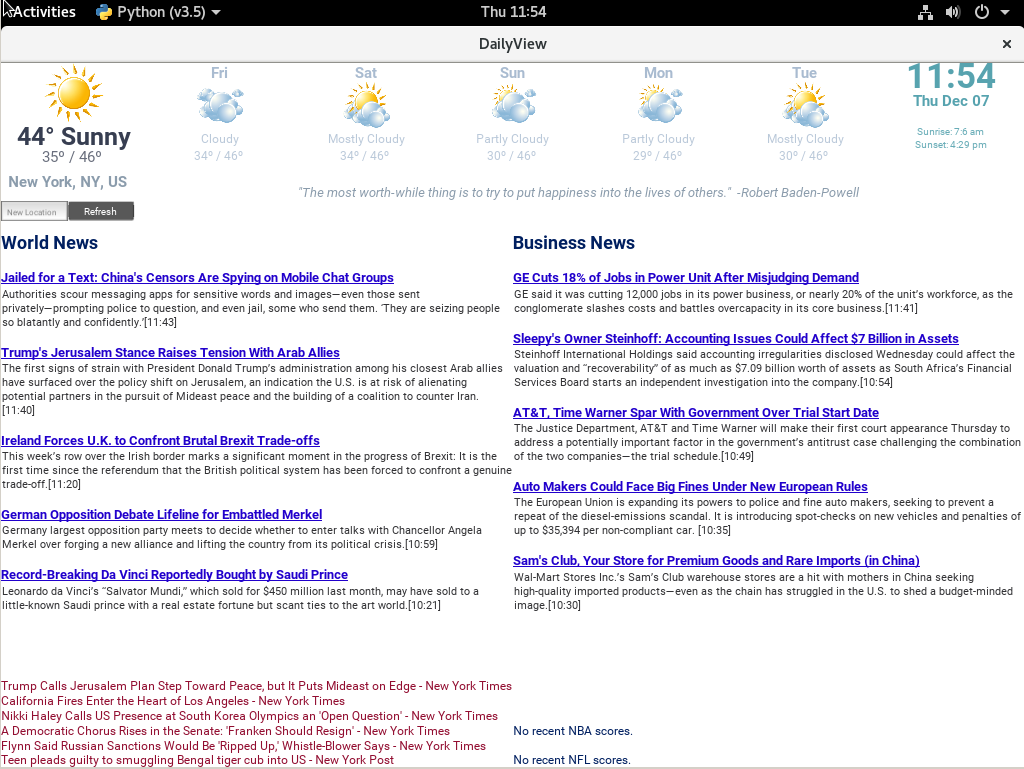
\includegraphics[width=\columnwidth]{images/monitor.png}
  \caption{Raspberry Pi IoT Application}
  \label{f:Figure1}
\end{figure}


As part of the display, a continuous running clock was added, which necessitated the application to be on a constant refresh. This was implemented successfully and at a relatively low cost with no significant delays. The total build of the application consumed 966,565 bytes with each refresh using just 1032 bytes. 
At the initialization of the program, the application uses the user's IP address to find their zip code to populate the local weather forecast and local news. For the weather, the user will get the current temperature with a high/low for the current day and each day in the five day forecast.

Additionally, as news stories are published to the WSJ news feed, they will be read into the application and refreshed. Stories are shown in chronological order along with their time stamp of publication and each is hyperlinked directly to the full story if the user wants more information. 

\subsection{Application to Big Data}
One of the main benefits of IoT is synthesizing data across numerous platforms and data sources into a desired output. Our desired output is a one-stop interface with interesting information that can be displayed anywhere with an outlet, internet connection and monitor. 

The various components of the monitor are only made possible by the creativity by the providers in solving difficult Big Data issues, such as the  clustering of news (Google) and weather forecasting (Yahoo/Weather Underground). Each provider's relationship to Big Data is worth examination and will be the topic of the following sections. 

\subsection{Google News}
\subsubsection{Big Data Description}
Google News has evolved into a central source of information for how a large share of the population receives its news. In fact, as a display of the trust that users place in Google to deliver the most information in the most efficient manner, it was found that users are more likely to trust a Google news headline than that same headline from the original source \cite{edelman}. Additionally, $44\%$ of users were found to read nothing more than the headlines \cite{googleheadlines}. This is a testament to their ability to simplify the universe of world news into succinct rankings. 

Entering into its fifteenth year, Google News aggregates from 50,000 news sources worldwide across 30 different languages. In 2012, they reported the division was receiving 1 billion unique visits a \emph{week}\cite{krishna}. For reference, major individual news providers, such as CNN and the New York Times receive 125 million and 99 million unique visitors per \emph{month} \cite{nytimes}. These statistics further demonstrate Google's successful navigation of the Big Data problem for news stories in the eyes of its users. 
It's relatively clear why this is an important Big Data problem, but one might be curious how they're able to effectively navigate the problem. Unfortunately, the full design from start to finish is a well kept secret, but pieces have been released and one can piece together a mosaic view of what might be going on under the hood. The decision to not disclose the techniques for ranking news stories is understandable, but it has been a lightening rod of controversy nonetheless. Some view the decision of Google's scoring as effectively acting as a censor for the internet while they maintain it is to keep the integrity of the algorithm so that news stories cannot be written purely for traffic, known as search engine optimization \cite{censor}. 

On the surface, one might question the economic value of Google News to the larger company since it is a free service for both users and providers. However, there is a tremendous amount to be gained in solving this Big Data problem. Even though Google does not show ads on its news site, it was estimated to generate spillover traffic into its search engine that leaves the News entity worth $\$100$ million in 2008 \cite{newsvalue}. The current valuation is undoubtedly higher, but it remains undisclosed. So while there are profits to be made for Google in this quest, publishers of these stories have a tremendous amount of interest in this problem as well. Some providers don't believe content should be indexed to Google's search algorithm for free and Google should pay them for their investigative research. One such provider, who happened to be Germany's largest news source, decided to remove themselves from the index for two weeks. The results were devastating for the site as traffic through the site dropped by $40\%$ \cite{springer}. It was a quick lesson in how critical positioning can be be in the Big Data world of news aggregation.

\subsubsection{Big Data Solution}
Just as news is constantly evolving, so are Google's solutions to this Big Data problem. As we've seen recently, news aggregation services are under pressure to become more intelligent on what news is shown in the hopes of preventing fake news from making it into the top results. 

The technical specifics of what Google is implemented has largely been kept under wraps, but we did learn a few of the techniques and platforms in 2007. In at least the early versions, Google used MinHash, Probabilistic Latent Semantic Indexing and Covisitation to solve this Big Data. Specifically, these methods will compare historical clicks with other similar users for recommendations, decipher key words and phrases from an article for grouping and track how news stories are clicked within a certain time frame to find stories that were read successively. For processing these queries, Google uses MapReduce and Hadoop architecture \cite{googlearch}.

For the inputs into these algorithms, Google will analyze several metrics of a provider to see how they should be ranked along with the user preferences. These metrics include things like how large the staff is, how many articles they put out, how many websites reference that news source (PageRank) and the breadth of news topics covered \cite{sauce}. 

\subsection{Weather Underground via Yahoo API}
\subsubsection{Big Data Description}
Weather is a primary concern in business planning for many industries, such as airlines or agriculture. As a result, companies are willing to dedicate a tremendous amount of resources towards accurate forecasts. One of the most innovative companies and a great example of the intersection of IoT and Big Data is Weather Underground. 

Weather Underground is a weather forecasting service that was once owned by the Weather Channel and recently, partially by IBM to integrate with its growing IoT ecosystem. What makes the company unique is how their forecasts are formulated. In their model,  they couple traditional forecasting tools with IoT. The traditional readings come from the National Weather Service (NWS), which aggregates data from airports and weather balloons. IoT has lead to a new dimension of forecasting as personalized weather stations are distributed to to its users for live forecasts in places that traditional instruments might not be available. As of now, they have 250,000 users set up on the platform. This setup provides an additional layer of information, yielding more frequent data, longer forecast windows and greater certainty for a given area. Namely, users can get new forecasts every 15 minutes (versus every 4 hours on the NWS) and forecasts up to two weeks in advance (compared to one week for NWS) \cite{wuabt}. This use of the IoT, specifically edge computing, which will be expanded on later, provides a tremendous example of how IoT can be used to enhance Big Data analysis. 

For those that choose to participate in the service, they will purchase a Personal Weather Station (PWS) that allows them to measure temperature, humidity, pressure, rainfall, wind speed and direction via sensors. The major advantage of the PWS comes from its pressure and wind metrics as users can get a better idea of humidity and wind chill, giving a more accurate representation of current conditions. Neither of these are available through the NWS. In the end, this amounts to around 3 billion data points for the Weather Underground model, servicing around 26 billion inquiries a day \cite{ibm}. This is a great demonstration of edge computing that was explained earlier for its ability to collect and process relevant information before sending it to the cloud for synthesis with other devices. 

\subsubsection{Big Data Solution}
To process its data in the past, which amounts to multiple terabytes daily, Weather Underground has stored its forecasts, radar data and satellite data using Apache Hadoop and Amazon Web Services \cite{wuinf}. In fact, IBM has stated a large reason for their motivation to have an ownership stake in the company was due to the cloud infrastructure that Weather Underground had built for fielding the massive volume of requests and forecasts it processes daily.  

\subsection{Limitations}

While this application shows what an IoT device can achieve with Big Data, the most influential uses of IoT come when devices are able to communicate with one another and create more data that can be implemented back into future improvements in the device, as we have seen. The limitation of this current program is that it is a singular instance of the application. Allowing multiple applications to be deployed where information can be collected on \emph{volunteered} information would be orders of magnitude more difficult to implement, but could be an interesting addition to gain better insight on the user base. Then, this data can be pooled together for how the application could be tailored to meet geographic or demographic preferences.

Additionally, with a large enough user base, we would be interested in tracking the number of downloads, active users and which panels of the display are clicked most often. All of these metrics can be readily accessed through integration with Google Analytics, which allows one to analyze different events within the application \cite{googleanalytics}.

\section{Conclusion}
As we've seen, IoT cannot realize its full potential without Big Data. The IoT universe represents the senses by which Big Data is collected for later insights and innovations. For this reason, the IoT revolution has the potential to completely change the world as we currently know. It could be a world in which automobile accidents are no longer a tragic reality or a world where health care delivers the most personalized plan with attention on every minute detail. Additionally, users are able to benefit from the increase in computing power per dollar spent, allowing them more flexibility than ever to design their own IoT device, as was demonstrated in the application made for this paper. However, against this rapid pace of innovation in IoT, some of its most attractive features of interdependency among devices expose the technology to some of its greatest vulnerabilities. Keeping this growth rate in the products in step with security will prove to be one of the biggest challenges in coming years. 

\appendix

\section{Code Compilation and Sample Output}
The following urls are intended to direct to various parts of the project. 
\begin{itemize}
    \item Packages required to compile the project along with sample input
        \begin{itemize}
            \item \url{https://github.com/bigdata-i523/hid334/tree/master/project}
        \end{itemize}
    \item Python code to create the monitor: 
        \begin{itemize}
            \item \url{https://github.com/bigdata-i523/hid334/blob/master/project/code/project.py}
        \end{itemize}
    \item Weather codes: 
        \begin{itemize}
            \item \url{https://github.com/bigdata-i523/hid334/blob/master/project/weathercodes.py}
        \end{itemize}
    \item Kivy file: 
        \begin{itemize}
            \item \url{https://github.com/bigdata-i523/hid334/blob/master/project/DailyView.kv}
        \end{itemize}
    
    
\end{itemize}
%https://www.csoonline.com/article/2130877/data-breach/the-16-biggest-data-breaches-of-the-21st-century.html

%https://www.networkworld.com/article/3166106/internet-of-things/4-critical-security-challenges-facing-iot.html

%http://www.eweek.com/security/consumers-want-iot-toys-regardless-of-security-survey-finds


%The paper should be 2 written pages excluding figures and references. For %your chosen topic, your paper should answer the following questions:
%Why is this topic important?
%How is it relevant to Big Data?
 
%More information on scope:
%You should assume not much knowledge, common knowledge is ok, but as you %have only 2 pages you need to make sure you address
 
%a) what is the problem
%b) why is big data involved
%c) how can big data or analytics of big data help
%d) what infrastructure/programs/systems exist for this
 
\begin{acks}
The author would like to thank Professor Dr. Gregor von Laszewski, Juliette Zerick and the other Associate Instructors for their support and suggestions in exploring this topic.
\end{acks}

\bibliographystyle{ACM-Reference-Format}
\bibliography{report} 

%\section{Issues}

\DONE{Example of done item: Once you fix an item, change TODO to DONE}

\subsection{Assignment Submission Issues}

    \TODO{Do not make changes to your paper during grading, when your repository should be frozen.}

\subsection{Uncaught Bibliography Errors}

    \TODO{Missing bibliography file generated by JabRef}
    \TODO{Bibtex labels cannot have any spaces, \_ or \& in it}
    \TODO{Citations in text showing as [?]: this means either your report.bib is not up-to-date or there is a spelling error in the label of the item you want to cite, either in report.bib or in report.tex}

\subsection{Formatting}

    \TODO{Incorrect number of keywords or HID and i523 not included in the keywords}
    \TODO{Other formatting issues}

\subsection{Writing Errors}

    \TODO{Errors in title, e.g. capitalization}
    \TODO{Spelling errors}
    \TODO{Are you using {\em a} and {\em the} properly?}
    \TODO{Do not use phrases such as {\em shown in the Figure below}. Instead, use {\em as shown in Figure 3}, when referring to the 3rd figure}
    \TODO{Do not use the word {\em I} instead use {\em we} even if you are the sole author}
    \TODO{Do not use the phrase {\em In this paper/report we show} instead use {\em We show}. It is not important if this is a paper or a report and does not need to be mentioned}
    \TODO{If you want to say {\em and} do not use {\em \&} but use the word {\em and}}
    \TODO{Use a space after . , : }
    \TODO{When using a section command, the section title is not written in all-caps as format does this for you}\begin{verbatim}\section{Introduction} and NOT \section{INTRODUCTION} \end{verbatim}

\subsection{Citation Issues and Plagiarism}

    \TODO{It is your responsibility to make sure no plagiarism occurs. The instructions and resources were given in the class}
    \TODO{Claims made without citations provided}
    \TODO{Need to paraphrase long quotations (whole sentences or longer)}
    \TODO{Need to quote directly cited material}

\subsection{Character Errors}

    \TODO{Erroneous use of quotation marks, i.e. use ``quotes'' , instead of " "}
    \TODO{To emphasize a word, use {\em emphasize} and not ``quote''}
    \TODO{When using the characters \& \# \% \_  put a backslash before them so that they show up correctly}
    \TODO{Pasting and copying from the Web often results in non-ASCII characters to be used in your text, please remove them and replace accordingly. This is the case for quotes, dashes and all the other special characters.}
    \TODO{If you see a figure and not a figure in text you copied from a text that has the fi combined as a single character}

\subsection{Structural Issues}

    \TODO{Acknowledgement section missing}
    \TODO{Incorrect README file}
    \TODO{In case of a class and if you do a multi-author paper, you need to add an appendix describing who did what in the paper}
    \TODO{The paper has less than 2 pages of text, i.e. excluding images, tables and figures}
    \TODO{The paper has more than 6 pages of text, i.e. excluding images, tables and figures}
    \TODO{Do not artificially inflate your paper if you are below the page limit}

\subsection{Details about the Figures and Tables}

    \TODO{Capitalization errors in referring to captions, e.g. Figure 1, Table 2}
    \TODO{Do use {\em label} and {\em ref} to automatically create figure numbers}
    \TODO{Wrong placement of figure caption. They should be on the bottom of the figure}
    \TODO{Wrong placement of table caption. They should be on the top of the table}
    \TODO{Images submitted incorrectly. They should be in native format, e.g. .graffle, .pptx, .png, .jpg}
    \TODO{Do not submit eps images. Instead, convert them to PDF}

    \TODO{The image files must be in a single directory named "images"}
    \TODO{In case there is a powerpoint in the submission, the image must be exported as PDF}
    \TODO{Make the figures large enough so we can read the details. If needed make the figure over two columns}
    \TODO{Do not worry about the figure placement if they are at a different location than you think. Figures are allowed to float. For this class, you should place all figures at the end of the report.}
    \TODO{In case you copied a figure from another paper you need to ask for copyright permission. In case of a class paper, you must include a reference to the original in the caption}
    \TODO{Remove any figure that is not referred to explicitly in the text (As shown in Figure ..)}
    \TODO{Do not use textwidth as a parameter for includegraphics}
    \TODO{Figures should be reasonably sized and often you just need to
  add columnwidth} e.g. \begin{verbatim}/includegraphics[width=\columnwidth]{images/myimage.pdf}\end{verbatim}

re


\end{document}
